\begin{figure*}[htbp]
    \centering
    \begin{tabular}{m{43mm} m{43mm} m{43mm} m{43mm} m{10mm}}
        \hspace{-3mm}
        \begin{minipage}[b]{\linewidth}
            \centering
            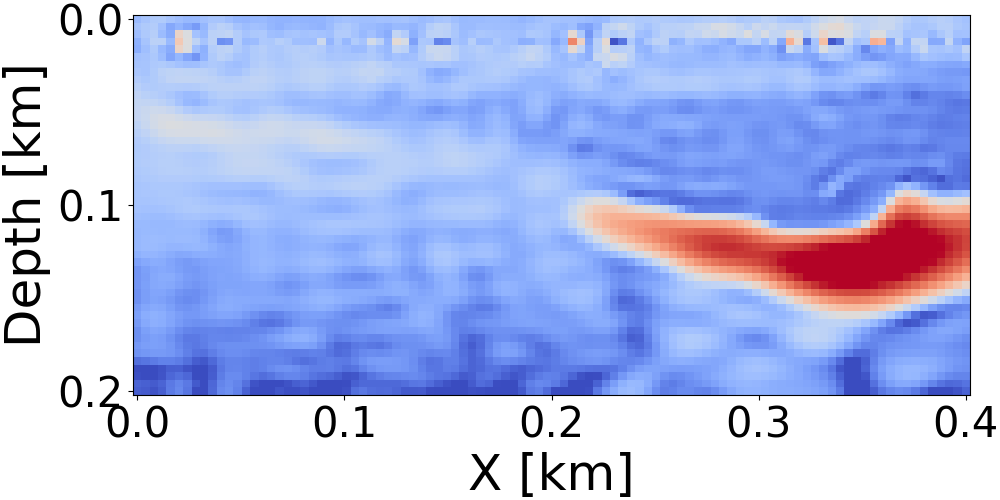
\includegraphics[width=\linewidth]{public/gradient_noisy}
            \vspace{-6mm}
            \caption*{Standard FWI}
            \vspace{1mm}
        \end{minipage} &
        \hspace{-8mm}
        \begin{minipage}[b]{\linewidth}
            \centering
            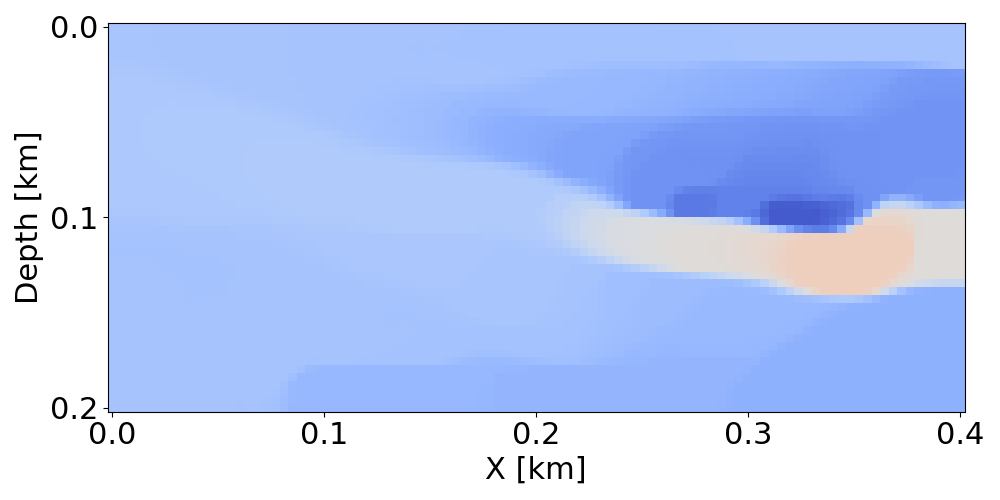
\includegraphics[width=\linewidth]{public/alpha_150_noisy}
            \vspace{-6mm}
            \caption*{Proposed, $\alpha = 150$}
            \vspace{1mm}
        \end{minipage} &
        \hspace{-13mm}
        \begin{minipage}[b]{\linewidth}
            \centering
            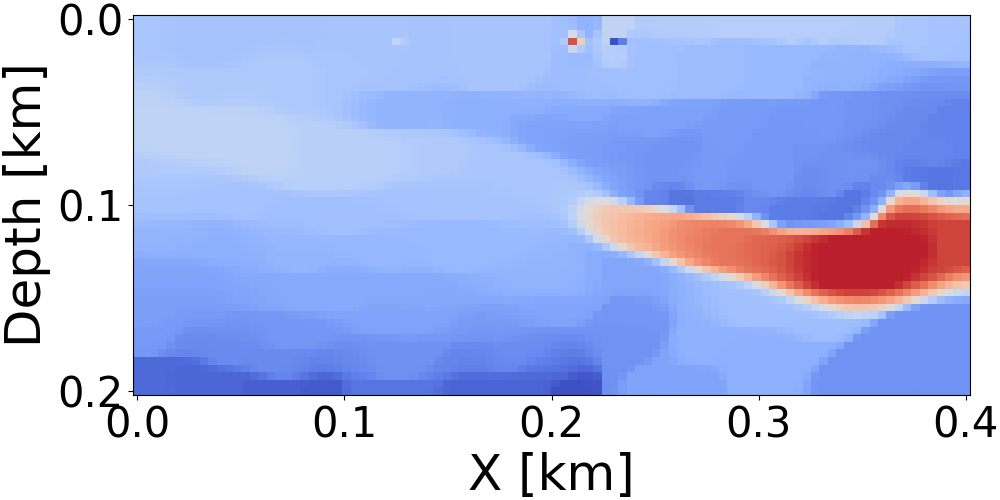
\includegraphics[width=\linewidth]{public/alpha_350_noisy}
            \vspace{-6mm}
            \caption*{Proposed, $\alpha = 350$}
            \vspace{1mm}
        \end{minipage} &
        \hspace{-18mm}
        \begin{minipage}[b]{\linewidth}
            \centering
            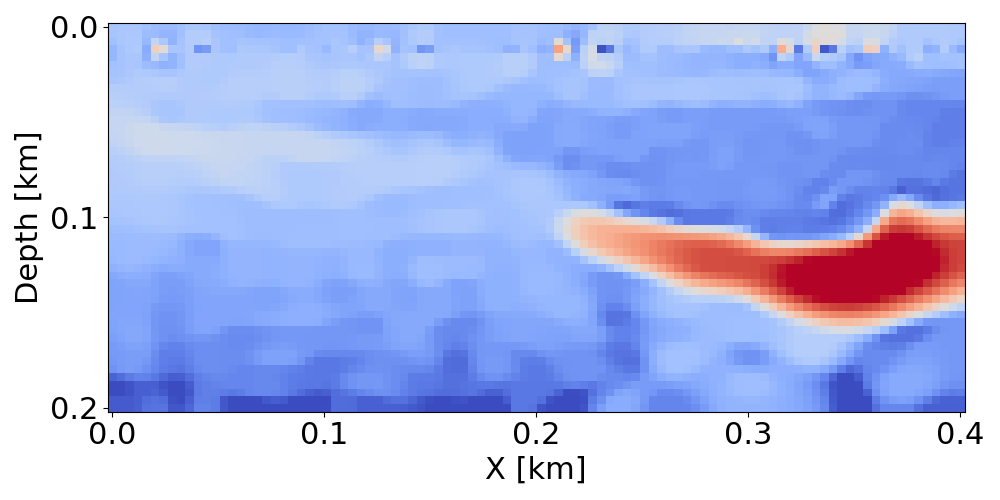
\includegraphics[width=\linewidth]{public/alpha_550_noisy}
            \vspace{-6mm}
            \caption*{Proposed, $\alpha = 550$}
            \vspace{1mm}
        \end{minipage} &
        \hspace{-21.5mm}
        \multirow[t]{3}{*}{\raisebox{-2.7mm}{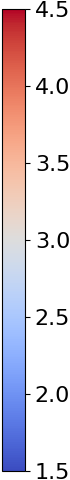
\includegraphics[height=40mm]{public/color-bar-min}}} \\
    \end{tabular}
    \vspace{-3mm}
    \caption{Velocity models [km/s] and their corresponding reconstructions. (with the noisy data)}
    \vspace{3mm}
    \label{fig:velocity-models-noisy}
\end{figure*}
